\documentclass[conference]{IEEEtran}
% If the IEEEtran.cls has not been installed into the LaTeX system files,
% manually specify the path to it.  e.g.
% \documentclass[conference]{./IEEEtran}

% Add and required packages here
\usepackage{graphicx,times,amsmath}

% Correct bad hyphenation here
\hyphenation{op-tical net-works semi-conduc-tor IEEEtran}

% To create the author's affliation portion using \thanks
\IEEEoverridecommandlockouts

\textwidth 178mm
\textheight 239mm
\oddsidemargin -7mm
\evensidemargin -7mm
\topmargin -6mm
\columnsep 5mm

\begin{document}

% Paper title: keep the \ \\ \LARGE\bf in it to leave enough margin.
\title{\ \\ \LARGE\bf Sample Paper for CIG'10: The 2010 IEEE
Conference on Computational Intelligence and Games \thanks{Ned Kelly
is with The Old Melbourne Gaol, Russell Street, Melbourne, Australia
(phone: +61-1-2345-6789; fax: +61-9-8765-4321; email: {\tt
Ned.Kelly@badboy.edu.au}).}}

\author{Ned Kelly, {\it Senior Member, IEEE}, Joe Byrne, {\it Member, IEEE}, and Steve Hart}

% Uncomment out the following line for invited papers
%\specialpapernotice{(Invited Paper)}

% Make the title area
\maketitle

\begin{abstract}
The abstract goes here.  Please try to make it less than 150 words.
We suggest that you read this document carefully before you begin
preparing your manuscript.  As the IEEE does not want conference papers
to contain keywords, ensure you do not include them in your paper.
Also, at this time, the IEEE only has some general guidelines about the
format for conference papers.  It is up to each individual conference
to decide which format to use.  In order to have a uniform look for all
papers published in the conference proceedings, we require that every
author follow the format of this sample paper.

This template is for LaTeX users and is based on the CEC'07 template
written by K.C. Tan. Many thanks go to him for his hard work.
Authors should use this sample paper as a guide in the production of
their paper. Word users should download and use the template files
posted on the conference website.
\end{abstract}

% No keywords

\section{Introduction}
% No \PARstart
If you have an introduction for your paper, put it here.

This sample file is intended to serve as a ``starter file.''  You
need to replace the text in this file with the text that makes up
your paper.

\subsection{Subsection Heading Here}
If applicable, subsection text goes here.  Note that you need to use
$\backslash$subsection.  You may or may not have any subsections.
That is okay.

\subsubsection{Subsubsection Heading}
Insert any subsubsection text here.  Same thing as before --- you may
or may not have any subsubsections.

\subsubsection{About This Template}
This template is for LaTeX users and is based on the CEC'07 template
written by K.C. Tan.  Many thanks go to him for his hard work.  Authors
should use this sample paper as a guide in the production of their paper.
Word users should download and use the template files posted on the
conference website.

\subsection{Page Layout}
\begin{itemize}
\item The IEEE now only accepts 100$\%$ Xplore compliant papers prepared
in PDF format.  Please make sure that you follow these guidelines in
preparing your PDF files.  Violations of any of these specifications
may result in the rejection of your paper.
\item Paper size: US letter format ($8.5\times 11$ in or $216\times
278$ mm).
\item Paper length: maximum 8 pages, including figures, tables, and
references.  In exceptional circumstances, up to two additional pages
will be permitted for a charge of USD\$100 per additional page.
\item Paper format: double column, single spaced, 10pt font.
\item Text width: 7.0 in (178 mm).
\item Text height: 9.375 in (240 mm).
All text and figures must be contained in the $178 \times 240$ mm
image area.
\item The left/right/bottom margin must be 0.75 in (19 mm).
\item The top margin must be 0.75 in (19 mm), except for the title page,
where it must be 1 in (25 mm).
\item Text should appear in two columns, each 3.4 in (86.5 mm) wide, with
0.2 in (5 mm) space between columns.
\item Do {\bf NOT} number the pages in the manuscript.
\item Unix LaTeX users should use the following commands to ``compile''
their paper:
    \begin{itemize}
    \item latex mypaper
    \item dvips -Ppdf -G0 -tletter mypaper.dvi
    \item ps2pdf -dEmbedAllFonts=true mypaper.ps mypaper.pdf
    \end{itemize}
\end{itemize}

The page size and margin settings in IEEEtran.cls are set for IEEE
Transactions papers.  Some adjustments have been made to produce this
sample paper.

{\it Also, please note, IEEE PDF eXpress will be made available to assist
in creating IEEE Xplore compliant PDF files for camera-ready submission.}

\section{Results}
The main results and findings go here.

Do not number an equation if it will not be directly cited
in the paper.  In order to avoid numbered equations, use
$\backslash$begin\{equation*\}--$\backslash$end\{equation*\},
$\backslash$[ --$\backslash$], or \$\$--\$\$.  For example:
\begin{equation*}
a = b + c,
\end{equation*}
$$\dot x = f(x,u) + g(x,u),$$
or
\[\ddot s=G(s,t)\]
where $f$, $g$, and $G$ are functions.

Note that Equation (\ref{equation-eqn1}) below is numbered!  It is
produced using $\backslash$begin\{equation\}--$\backslash$end\{equation\}:
\begin{equation}
F_i(P_i)=a_{i}+b_{i}P_i+c_{i}P_{i}^2
\label{equation-eqn1}
\end{equation}
where $a_{i},\ b_{i}$, and $c_{i}$ are coefficients of unit $i$, and $P_i$
represents some value for unit $i$.

Aligning equations can be done with
either the align or eqnarray commands.  Recently,
$\backslash$begin\{align\}--$\backslash$end\{align\} has gained popularity
over $\backslash$begin\{eqnarray\}--$\backslash$end\{eqnarray\}.

Equation (\ref{equation-eqn2}) is produced using
$\backslash$begin\{align\}--$\backslash$end\{align\}:
\begin{align}
\dot {x}_l=& \sum_{i = 1}^m {\frac{c_{P_{x_i} } e^{k_{x_i}\bar{x}_i} + c_{N_{x_i} }
e^{ -  k_{x_i} \bar{x}_i}}{e^{k_{x_i} \bar{x}_i} + e^{ - k_{x_i} \bar{x}_i}}} \nonumber\\
& + \frac{1}{2}\sum\limits_j^q (c_{P{u_j }} + c_{N _{u_j }} ) \nonumber\\
y=& \ A_0 + A_1 \tanh (K_x \bar {x}) + B\tanh (K_u \bar {u}) \nonumber\\
 =& \ F(x),
\label{equation-eqn2}
\end{align}
where $F(x)$ is a function.

Equation (\ref{equation-eqn3}) represents the same equation produced
using $\backslash$begin\{eqnarray\}--$\backslash$end\{eqnarray\}:
\begin{eqnarray}
\dot {x}_l&=& \sum_{i = 1}^m {\frac{c_{P_{x_i} } e^{k_{x_i}\bar{x}_i} + c_{N_{x_i} }
e^{ - k_{x_i} \bar{x}_i}}{e^{k_{x_i} \bar{x}_i} + e^{ - k_{x_i} \bar{x}_i}}} \nonumber\\
&&+ \frac{1}{2}\sum\limits_j^q (c_{P{u_j }} + c_{N _{u_j }} ) \nonumber\\
y&=& \ A_0 + A_1 \tanh (K_x \bar {x}) + B\tanh (K_u \bar {u})\nonumber\\
&=& \ F(x),
\label{equation-eqn3}
\end{eqnarray}
where $F(x)$ is a function.  You get the idea!

\subsection{Example of a Figure}
Below is an example of a floating figure using the graphicx
package.  Note that $\backslash$label must occur AFTER (or within)
$\backslash$caption.  For figures, $\backslash$caption should occur
after the $\backslash$includegraphics.  To reference a figure, use
the word Figure followed by the figure number.  Here is an example:
Figure~\ref{figure-fig1}.

\begin{figure}[htp]
\centerline{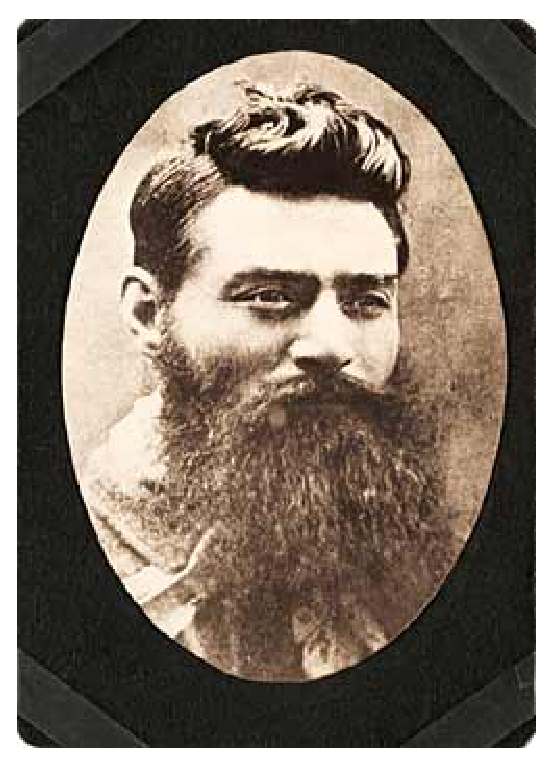
\includegraphics[width=0.6\columnwidth]{NedKelly.eps}}
\caption{A famous Australian bush-ranger: Ned Kelly}
\label{figure-fig1}
\end{figure}

\subsection{Figures and Tables}
Please follow the style in this sample paper when generating your figures
and tables.

\subsection{What Sections to Include}
Usually, your paper should contain an Introduction, Background,
Methodology, Results, and Conclusions section.  You may also add
Acknowledgments if you like.  After that, you should list your references
in a References section.

\subsection{Page Limit and Overlength Page Charges}
A paper submitted to this conference should be prepared in a
single-spaced, two-column format.  Its length must be kept to 8
pages or less.  In exceptional circumstances, up to two additional
pages will be permitted for a charge of USD\$100 per additional page.
Table~\ref{table-tab1} shows the page limit and page charge schedule.

% An example of a floating table.  Note that, for IEEE style tables, the
% \caption command should come BEFORE the table.  Table text will default
% to \footnotesize as IEEE normally uses this smaller font for tables.
% The \label must come after \caption as always.
\begin{table}
\begin{center}
%% Increase table row spacing; adjust to taste
\renewcommand{\arraystretch}{1.3}
\caption{Page Limit}
\label{table-tab1}
% The array package and the MDW tools package offers better commands
% for making tables than plain LaTeX2e's tabular which is used here.
\begin{tabular}{|c|c|}
\hline
Page limit: & 8\\
\hline
Excess page charge: & USD\$100/page\\
\hline
\end{tabular}
\end{center}
\end{table}

Another example of a table is shown in Table~\ref{table-tab2}.

\begin{table}[h]
\caption{A second table}
\begin{center}
\begin{tabular}{|c|c|c|c|c|c|}
\hline
\multicolumn{1}{|c|}{\raisebox{-1.50ex}[0cm][0cm]{\!Method\!}}
& \multicolumn{1}{|c|}{Mean}
& \multicolumn{1}{|c|}{Best}
& \multicolumn{1}{|c|}{Mean}
& \multicolumn{1}{|c|}{Maximum}
& \multicolumn{1}{|c|}{Minimum} \\
& time & time & cost & cost & cost\\ \hline
A      &  $928.36$  &  $926.20$  &  $124793.5$ & $126902.9$ & $123488.3$ \\ \hline
B      &  $646.16$  &  $644.28$  &  $124119.4$ & $127245.9$ & $122679.7$ \\ \hline
C      &  $1056.8$  &  $1054.2$  &  $123489.7$ & $124356.5$ & $122647.6$ \\ \hline
D      &  $632.67$  &  $630.36$  &  $123382.0$ & $125740.6$ & $122624.4$ \\ \hline
\end{tabular}
\label{table-tab2}
\end{center}
\end{table}

Citations are included like so~\cite{book}.
Multiple citations appear like this~\cite{conf,article}.

\section{Conclusions}
The conclusion goes here.

This template is for LaTeX users. This CIG'10 LaTeX template is
based on the CIG'08 template written by Luigi Barone and the CEC'07
template written by K.C. Tan. Many thanks go to them for their hard
work. Authors should use this sample paper as a guide in the
production of their paper. Word users should download and use the
template files posted on the conference website.

% Conference papers do not normally have an appendix, but if you must,
% use \section*
\section*{Appendix}
Put your appendix here if you have any.

% Use \section* for the acknowledgments
\section*{Acknowledgments}
The authors would like to thank Mr. XYZ for his/her help.
This work was supported in part by the National Science Foundation
under grant no. XXXXX, etc.

% Trigger a \newpage just before a given reference number in order to
% balance the columns on the last page.  Adjust the value as needed;
% it may need to be readjusted if the document is modified later.
%\IEEEtriggeratref{8}
% The "triggered" command can be changed if desired:
%\IEEEtriggercmd{\enlargethispage{-5in}}

% The references section can either be generated by hand or by an
% automatic tool like BibTeX.  If using BibTex, use the standard IEEEtran
% bibliography style.
%\bibliographystyle{IEEEtran.bst}
%
% The argument to \bibliography is/are the name(s) of your BibTeX file(s)
% that contains string definitions and bibliography database(s).
%\bibliography{IEEEabrv,SamplePaper}
%
% If you generate the bibliography by hand, or if you copy in the
% resultant .bbl file, set the second argument of \begin to the number of
% references in the bibliography (used to reserve space for the reference
% number labels box).

\begin{thebibliography}{3}
\bibitem{book}
A.~Great, \emph{This is the book title}.\hskip 1em plus 0.5em minus 0.4em\relax
  This is the name of the publisher, 2006.

\bibitem{conf}
F.~Author, S.~Author, and T.~NonRelatedAuthor, ``This is the paper title,'' in
  \emph{This is the proceedings title}, 2008, pp. 1--8.

\bibitem{article}
B.~Myself, ``This is the title of the journal article,'' \emph{This is the name
  of the journal}, pp. 1--30, 2007.
\end{thebibliography}

% That's all folks...
\end{document}
